\documentclass{article}

% Useful packages
\usepackage{amsmath}
\usepackage{algorithm}
\usepackage{algorithmic}
\usepackage{graphicx}
\usepackage[colorlinks=true, allcolors=blue]{hyperref}
\usepackage{listings}
\usepackage{xskak}
\usepackage[french]{babel}
\usepackage[utf8]{inputenc}

\usepackage{caption}
\DeclareUnicodeCharacter{2009}{\times}

%%%%%%%%%%%%%%%% Lengths %%%%%%%%%%%%%%%%
\setlength{\textwidth}{16.5cm}
\setlength{\evensidemargin}{0.5cm}
\setlength{\oddsidemargin}{0.5cm}

%%%%%%%%%%%%%%%% Variables %%%%%%%%%%%%%%%%
\def\projet{4}
\def\titre{Systèmes d'équations non linéaires}
\def\groupe{1}
\def\equipe{3}
\def\responsible{melkhader}
\def\secretary{ahermitte}
\def\others{alagraoui001 ,stakaguessu}

\begin{document}


%%%%%%%%%%%%%%%% Header %%%%%%%%%%%%%%%%
\noindent\begin{minipage}{0.98\textwidth}
  \vskip 0mm
  \noindent
  { \begin{tabular}{p{7.5cm}}
      {\bfseries \sffamily
        Projet \projet} \\ 
      {\itshape \titre}
    \end{tabular}}
  \hfill 
  \fbox{\begin{tabular}{l}
      {~\hfill \bfseries \sffamily Groupe \groupe\ - Equipe \equipe
        \hfill~} \\[2mm] 
      Responsable : \responsible \\
      Secrétaire : \secretary \\
      Codeurs : \others
    \end{tabular}}
  \vskip 4mm ~

  ~~~\parbox{0.95\textwidth}{\small \textit{Résumé~:} \sffamily Le but de ce projet consiste à programmer des algorithmes dédiés à la recherche de racines d'équations non linéaires. La méthode utilisée est la méthode de Newton-Raphson, et l'objectif c'est d'évaluer la qualité d'une telle solution en l'appliquant dans la construction de quelques algorithmes notamment le calcul de points d'équilibre électrostatique et la méthode de Bairstow. }
  \vskip 1mm ~
\end{minipage}

\section{Solveur Newton-Raphson}
La méthode de Newton-Raphson consiste à chercher une racine d'une fonction $f : \mathbb{R}^n \rightarrow \mathbb{R}^m$ dérivable sur l'intervalle d'étude, en se basant sur le calcul de la pente de $f$ en un vecteur de départ $U_0 \in \mathbb{R}^n$ choisi arbitrairement.

\subsection{Choix du pas}
 On choisit un pas représenté par un vecteur $V$ tel que $f(U+V) = 0_m$. Pour calculer $V$, la matrice jacobienne $H(f,U)\in \mathbb{M}_{m,n}(\mathbb{R})$ associée à la fonction en ce point est obtenue en calculant $\frac{\partial f_i}{\partial u_j}$. $V$ est alors calculé en résolvant l'équation $f(U+V) = 0$, où $f(U+V)$ est approximé par $f(U) + H\times V$. On obtient l'équation $f(U+V) = f(U) + H\times V$. Pour trouver $V$, il s'agit donc de résoudre le système linéaire $H\times V = -f(U)$.
 
 \subsection{Résolution de l'équation}
 On cherche un point $U$ tel que $f(U) = 0$ à partir d'un point de départ $U_0$. L'algorithme de Newton-Raphson consiste donc à calculer $V$ de manière à ce que $f(U+V)$ se rapproche de 0. Tant que la valeur de $V$ n'est pas telle que $f(U+V) = 0$, on itère sur $U$ en transformant $U$ en $U+V$ et on recalcule $V$ en résolvant le système linéaire précédemment énoncé. Dû au problème de la précision machine qui ne permet pas la comparaison de $f(U+V)$ avec 0, l'algorithme s'achève quand $|f(U+V) - f(U)| < \epsilon$, où $\epsilon$ est un paramètre pris en entrée de la fonction Newton\_Raphson(). Afin de s'assurer que l'on ne diverge pas, la fonction prend aussi en paramètre le nombre d'itérations maximale pour trouver $U$ tel que $f(U) = 0$.
 \subsection{Backtracking}
 Afin de s'assurer que l'algorithme n'a pas dépassé la racine lors de son déroulement, on utilise la technique de backtracking. Celle-ci consiste à vérifier la réduction de la norme de $f(U)$ à chaque itération de la boucle principale. Ainsi, si la norme de $f(U+V)$ devient supérieure à celle de $f(U)$ (ce qui indique le dépassement de la racine), le pas $V$ est multiplié par un facteur de réduction tant que $|f(U+V)| > |f(U)|$. De cette manière, la nouvelle version de l'algorithme de Newton-Raphson assure que l'on ne dépasse pas la racine. En utilisant la méthode du backtracking, nous pouvons contrôler la taille des sauts effectués par l'algorithme, ce qui peut améliorer la convergence de la méthode.
 \subsection{Trajectoire de convergence}
Pour tester l'algorithme de Newton-Raphson , nous l'avons appliqué à des fonctions non-linéaires de plusieurs variables. Nous avons utilisé la méthode de Newton-Raphson pour résoudre une fonction non-linéaire en 3 dimensions et au même temps nous traçons la trajectoire de convergence en 3D comme l'illustre la figure~\ref{fig:convergence}. La fonction non-linéaire utilisée est $f(x,y,z) = (x^2 + y^2 - z, x + y - z^2, \sin(x) + \cos(y) - z)$. Nous avons utilisé une version modifiée de l'algorithme qui permet à la fois de trouver la racine de la fonction et enregistrer la trajectoire de convergence. Enfin, nous avons tracé la trajectoire de convergence en rouge sur les surfaces des trois fonctions en 3D. 

Le choix de cette fonction est justifié par sa complexité et sa non-linéarité. En effet, elle contient une combinaison de termes quadratiques et trigonométriques, ce qui la rend plus difficile à résoudre analytiquement et nécessite donc l'utilisation d'une méthode numérique.


\begin{figure}[h]
    \centering
    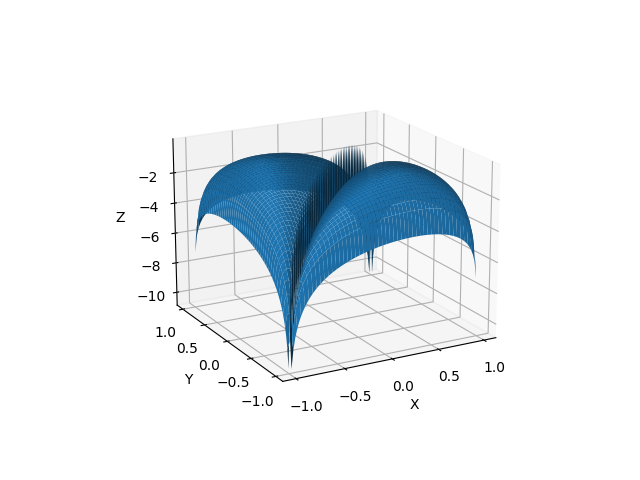
\includegraphics[width=0.8\textwidth]{Figure_1.png}
    \caption{Trajectoire de convergence de Newton-Raphson}
    \label{fig:convergence}
\end{figure}

Pour la fonction $f(x,y,z) = (x^2 + y^2 - z, x + y - z^2, \sin(x) + \cos(y) - z)$, nous avons choisi de tracer les surfaces $Z_1 = X^2 + Y^2$, $Z_2 = X + Y$ et $Z_3 = \sin(X) + \cos(Y)$. Bien que ces surfaces ne correspondent pas exactement à la fonction étudiée, elles permettent de visualiser la trajectoire de convergence de manière claire et lisible, ce qui facilite la compréhension de la représentation graphique. Il est important de noter que le choix de ces surfaces n'affecte pas la précision de l'algorithme de Newton-Raphson et leurs choix dépend de la fonction étudiée. Enfin, nous avons tracé la trajectoire de convergence en rouge sur ces surfaces, ce qui nous permet de suivre visuellement la convergence de l'algorithme vers la racine de la fonction. On peut observer que l'algorithme converge rapidement vers la racine, et que le chemin emprunté par l'algorithme est relativement direct, ce qui indique que l'algorithme a trouvé la racine efficacement.

\section{Équilibre éléctrostatique}
\subsection{Les points d'équilibre }
Cette partie consiste à étudier les positions d’équilibre d’un système composé de deux charges
électrostatiques situées en 1 et -1. En supposant qu'il existe $N$ charges positionnées à $x_{1}, x_{2}, ....x_{N}$ dans l'intervalle $[-1, 1]$, l'objectif est de trouver la position d'équilibre de ce système.
L'énergie totale de ce système est s'exprime: 
\[ E(x_{1}, x_{2} , ... , x_{N}) = \sum _{i=1}^{N} \left( log|x_{i} + 1|+ log|x_{i} - 1| + \frac{1}{2} \sum _{j=1, j\neq i}^{N} log|x_{i} - x_{j}| \right )\]
Une position d'équilibre est une position pour laquelle l'énergie présente un extremum, ainsi il faut résoudre le système d'équations suivant: $\nabla E(x_{1}, x_{2} , ... , x_{N}) = 0_{N}$. Pour cela on calcule d'abord l'expression explicite de la fonction $\nabla E(x_{1}, x_{2} , ... , x_{N})$ et de son jacobien, et par suite on lui appliquer la méthode de Newton-Raphson.
Puisque E est continue et dérivable sur $]-1,1[$ et suppose que toutes les positions des $N$ charges sont deux à deux distinctes alors on peut calculer la dérivée partielle de E en $x_{i}$:
\[\frac{\partial E}{\partial x_{i}} = \frac{1}{x_{i} + 1}  + \frac{1}{x_{i} - 1} + \frac{1}{2} \sum _{j=1, j\neq i}^{N} \frac{1}{x_{i} - x_{j}}\]
On gardant les mêmes hypothèses sur les positions des charges, les coefficients de la matrice jacobienne de $\nabla E(x_{1}, x_{2} , ... , x_{N})$ s'expriment pour tout $1\leq i,j \leq N$:
\[
\begin{cases}
    \text{si } i=j:  &\displaystyle\frac{\partial E}{\partial x_{i}^{2}} = -\frac{1}{(x_{i} + 1)^{2}}  - \frac{1}{(x_{i} - 1)^{2}} - \frac{1}{2} \sum _{j=1, j\neq i}^{N} \frac{1}{(x_{i} - x_{j})^{2}} \\
    \text{si } i\neq j : & \displaystyle\frac{\partial E}{\partial x_{i}\partial x_{j}} = \frac{1}{2(x_{i} - x_{j})^{2}} 
\end{cases}
\]
\subsection{Lien avec les polynômes de Legendre}
La figure~\ref{fig:legendre} montre le résultat de l'application de l'algorithme sur un vecteur de positions de 10 charges choisies aléatoirement dans $]-1,1[$ (représentés par des croix ), ainsi que les courbes représentatives des fonctions dérivées, des polynômes de legendre de degré entre 2 et 6. 

Sur cet exemple, on remarque que les polynômes de legendre de degré 5,2,4 et 3 ont des racines qui coïncident avec les points d'équilibre trouvés. En effet, les polynômes de Legendre permettent de déterminer les positions d'équilibre des charges électriques en résolvant l'équation de Laplace-Poisson pour trouver le potentiel électrostatique dans le système, puis en utilisant les coefficients des polynômes de Legendre pour déterminer les positions où les forces électrostatiques nettes sur toutes les charges sont nulles.
\begin{figure}[h]
    \centering
    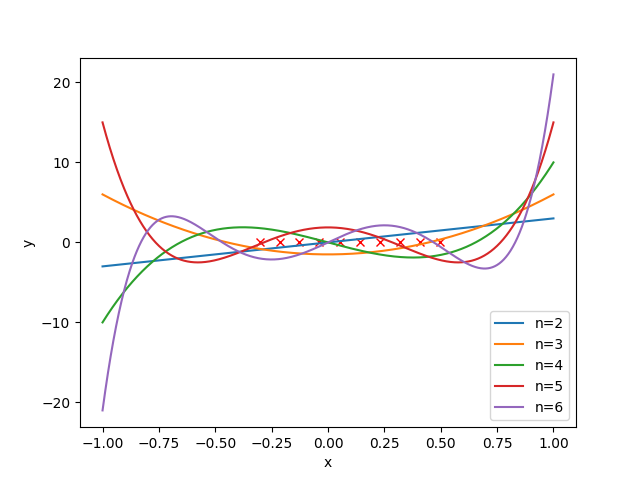
\includegraphics[width=15cm, height = 9cm]{Legendre.png}
    \caption{Les points d'équilibre et les polynômes de legendre}
    \label{fig:legendre}
\end{figure}
\newpage
Finalement, les éléments diagonaux de la matrice jacobienne de $\nabla E(x_{1}, x_{2} , ... , x_{N})$  sont négatives. En effet, comme c'est expliqué précédemment, ceux-ci correspondent aux dérivées secondes de $E$. Ainsi, puisqu’elles sont négatives, les solutions représentent un maximum d’énergie.







\section{Factorisation polynomiale de Bairstow}
La méthode de Bairstow est une méthode itérative qui permet de factoriser des polynômes de haut degré en utilisant la méthode de Newton-Raphson. Elle est également utilisée pour trouver les racines réelles d'un polynôme en utilisant des approximations des racines. Cependant, cet algorithme ne permet pas de trouver les racines complexes. Dans cette partie, on s'intéresse à une version modifiée de cette méthode qui permet de les trouver en se basant sur la méthode de Newton-Raphson.
\subsection{Implémentation de l'algorithme }
Soit un polynôme $P$ de degré $1 \leq n$ à coefficients réels. On sait que $P$ est scindé dans $C$, alors si il admet une racine complexe $\lambda$ alors il peut se factoriser comme suit : 
$P(X) = (X^{2} + 2\Re(\lambda) + |\lambda|^{2})^{m_{\lambda}} H(X)$ avec $m_{\lambda}$ la multiplicité de $\lambda$ et $H$ un polynôme de degré $n - 2\times m_{\lambda}$.

La variante de Bairstow utilisée consiste à faire des divisions successives du polynôme $P$ par une forme quadratique. En général, le reste de la division euclidienne de $P$ par une forme quadratique est un polynôme de degré 1, ainsi on peut exprimer $P$ comme suit:
$P(X) = (X^{2} + BX + C)Q(X) + RX + S$ où $B, C$ sont les coefficients de la forme quadratique et $Q$ et $RX + S$ le quotient et le reste de la division euclidienne. Si le reste de la division est nul partout, alors le polynôme de degré 2 divise $P$ ainsi on peut trouver les racines de $P$.
Pour cela, on considère que les coefficients $R$ et $S$ sont des fonctions en $B$ et $C$. Par suite, on pose la fonction à deux variables $F$ telle que: $ F(B, C) = \begin{pmatrix} R(B,C) \\ S(B,C) \end{pmatrix}$ avec $R$ et $S$ définies sur $\mathbb {R} \times [0, +\infty[ $.

Afin de déterminer la matrice jacobienne de $F$, on effectue une deuxième division euclidienne de $Q(X)$ par la même forme quadratique et par suite $Q$ s'exprime $Q(X) = (X^{2} + BX + C)Q_{1}(X) + R_{1}X + S_{1}$. Finalement la matrice jacobienne de $F$ est la suivante  : 
\[ J_{F}(B, C) = 
\begin{pmatrix} 
\frac{\partial R(B,C)}{\partial B} & \frac{\partial S(B,C)}{\partial C}
\\
\frac{\partial R(B,C)}{\partial B} & \frac{\partial S(B,C)}{\partial C}
\end{pmatrix} = 
\begin{pmatrix} 
B\times R_{1} - S_{1} & C\times R_{1}
\\
-R_{1}& - S_{1}
\end{pmatrix}
\] 

L'étape suivante est l'utilisation de la méthode de Newton-Raphson pour déterminer les zéros de la fonction $F$ car cela nous permet de trouver les racines complexes de $P$. En effet, soit $(B_{0}, C_{0})$ un zéro de $F$, alors le polynôme de degré 2 $X^{2} + B_{0}X + C_{0}$ divise $P$. Et par analogie avec la première formule factorisée de $P$, on a ces deux relations pour une racine complexe $\lambda$: $B_{0} = 2\Re(\lambda)$ et $C_{0} = |\lambda|^{2} = {\Re(\lambda)}^{2} + {\Im(\lambda)}^{2}$. \\ Ensuite, la résolution de ce système donne naissance à deux racines complexes conjuguées :
\[\begin{cases}
\lambda_{+} = \frac{B_{0}}{2} + i\sqrt{C_{0} - \frac{{B_{0}}^{2}}{4}} \\
\lambda_{-}= \frac{B_{0}}{2} - i\sqrt{C_{0} - \frac{{B_{0}}^{2}}{4}}
\end{cases}
\]
Finalement, de manière itérative on peut trouver toutes les racines de $P$, il suffit de continuer à faire des divisions euclidiennes par des formes quadratiques. Cependant, l'algorithme ne retourne pas toujours l'ensemble des racines ou parfois il retourne uniquement les racines réelles de $P$. Et cela est du au choix du vecteur de départ de l'algorithme de Newton-Raphson, en effet à chaque itération la méthode de calcul des zéros ne converge pas toujours.

\subsection{Comparaison des résultats}
La figure~\ref{compae_results} montre les racines obtenues par l'algorithme de Bairstow-Raphson implémentée, dans le plan complexe. Le polynôme utilisé ici est $P(X)=-12X^{7} + 2X^{6} + 3X^{5} -6X^{4}+ 6X^{3} -X^{2} + 5X -2$. Les résultats théoriques qu'on considère comme exactes sont obtenues par la fonction $roots$ de la bibliothèque $numpy$.
Il est à noter que sur certains polynômes, les résultats divergent et donnent des valeurs non entières $nan$, et cela dépend à la fois des valeurs initiales des coefficients de la forme quadratique et aussi du choix du vecteur de départ pour l'algorithme de Newton-Raphson. Pour minimiser ces erreurs, on a implémenter une fonction qui fabrique un bon vecteur de départ pour lequel la méthode de Newton converge.

\newpage
\begin{figure}[ht]
    \centering
    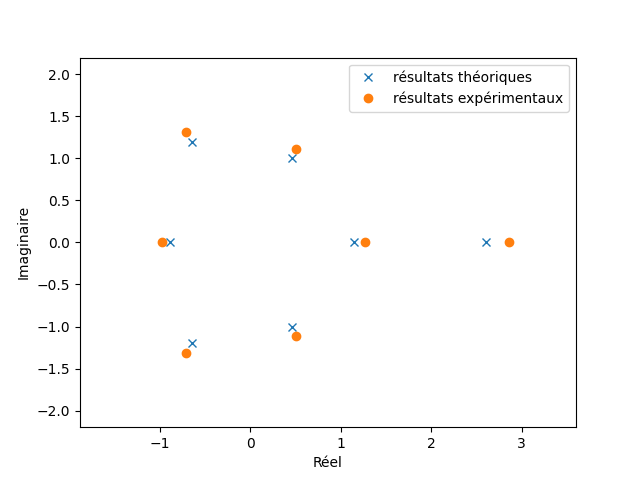
\includegraphics[width = 12cm, height = 8cm]{compare_results.png}
    \caption{Résultats de l'application de l'algorithme}
    \label{compae_results}
\end{figure}


\section{Conclusion}
 En guise de conclusion, ce projet a présenté la mise en œuvre et l'application de la méthode de Newton-Raphson pour résoudre des problèmes non linéaires. Nous avons examiné le solveur Newton-Raphson, son amélioration grâce au backtracking et la visualisation des trajectoires de convergence. De plus, nous avons exploré l'application de cette méthode pour trouver les points d'équilibre électrostatique et la factorisation polynomiale à l'aide de la méthode de Bairstow. Les résultats obtenus démontrent l'efficacité et la flexibilité de la méthode de Newton-Raphson pour aborder diverses applications dans la résolution d'équations non linéaires et mettent en évidence l'importance de l'optimisation des algorithmes pour assurer la convergence et la précision des solutions.

\end{document}
